\newpage
\section{Tiered compilation thresholds}
\label{a:compilethresholds}
\begin{table}[h]
  \centering
 % \caption{}
  \label{t:compilethresholds}
  \begin{center}
    \begin{tabular}{| l | p{9.0cm} | r | }
       \hline
       \textbf{flag} & \textbf{description} & \textbf{default} \\ \hline\hline
       CompileThresholdScaling & number of interpreted method invocations before (re-)compiling & 1.0\\ \hline
       Tier0InvokeNotifyFreqLog & Interpreter (tier 0) invocation notification frequency & 7\\ \hline
       Tier2InvokeNotifyFreqLog & C1 without MDO (tier 2) invocation notification frequency & 11 \\ \hline
       Tier3InvokeNotifyFreqLog & C1 with MDO profiling (tier 3) invocation notification frequency & 10 \\ \hline
       Tier23InlineeNotifyFreqLog & Inlinee invocation (tiers 2 and 3) notification frequency & 20 \\ \hline
       Tier0BackedgeNotifyFreqLog & Interpreter (tier 0) invocation notification frequency & 10 \\ \hline
       Tier2BackedgeNotifyFreqLog & C1 without MDO (tier 2) invocation notification frequency & 14 \\ \hline
       Tier3BackedgeNotifyFreqLog & C1 with MDO profiling (tier 3) invocation notification frequency & 13 \\ \hline
       Tier2CompileThreshold & threshold at which tier 2 compilation is invoked & 0 \\ \hline
       Tier2BackEdgeThreshold & Back edge threshold at which tier 2 compilation is invoked & 0 \\ \hline
       Tier3InvocationThreshold & Compile if number of method invocations crosses this threshold & 200 \\ \hline
       Tier3MinInvocationThreshold & Minimum invocation to compile at tier 3 & 100 \\ \hline
       Tier3CompileThreshold & Threshold at which tier 3 compilation is invoked (invocation minimum must be satisfied) & 2000 \\ \hline
       Tier3BackEdgeThreshold & Back edge threshold at which tier 3 OSR compilation is invoked & 60000 \\ \hline
       Tier4InvocationThreshold & Compile if number of method invocations crosses this threshold & 5000 \\ \hline
       Tier4MinInvocationThreshold & Minimum invocation to compile at tier 4 & 600 \\ \hline
       Tier4CompileThreshold & Threshold at which tier 4 compilation is invoked (invocation minimum must be satisfied) & 15000 \\ \hline
       Tier4BackEdgeThreshold & Back edge threshold at which tier 4 OSR compilation is invoked & 40000 \\ \hline
    \end{tabular}
  \end{center}
\end{table}
\newpage
\section{Cached profile example}
\label{a:cacheprofileexample}
\begin{lstlisting}[caption=Example of cached profiling information,label=l:cacheprofileexample,language=Java]
# 189 ciObject found
ciMethod java/lang/Double toString (D)Ljava/lang/String; 25 1 7 0 0
ciMethod java/lang/Long toString (J)Ljava/lang/String; 9 1 3 0 0
ciMethod java/lang/Long valueOf (J)Ljava/lang/Long; 25 1 7 0 0
ciMethod java/lang/Long longValue ()J 9 1 3 0 -1
ciMethodData java/lang/Double toString (D)Ljava/lang/String; 1 7 orig 280 152 101 83 95 3 127 0 0 88 140 138 72 3 127 0 0 144 1 0 0 0 0 0 0 0 0 0 0 0 0 0 0 0 0 0 0 0 0 0 0 0 0 0 0 0 0 0 0 0 0 0 0 0 0 0 0 0 0 0 0 0 0 0 0 0 0 0 0 0 0 0 0 0 0 0 0 0 0 0 0 77 68 79 32 101 120 116 114 97 32 100 97 116 97 32 108 111 99 107 0 0 0 0 0 0 0 0 0 0 0 0 0 0 0 0 0 0 0 0 0 0 0 0 0 0 0 0 0 0 0 0 0 0 0 0 0 0 0 0 0 0 0 0 0 0 0 0 0 0 0 0 0 0 0 0 0 0 0 0 0 0 0 0 0 0 0 0 0 0 0 0 0 0 0 0 0 0 0 0 0 0 0 0 0 0 0 0 0 0 0 0 0 0 0 0 0 0 0 0 0 0 0 0 0 0 0 0 0 0 0 0 0 0 0 0 0 3 0 0 0 33 0 0 0 1 0 0 0 0 0 0 0 0 0 0 0 0 0 0 0 248 3 0 0 248 31 0 0 2 0 0 0 0 0 0 0 0 0 0 0 48 0 0 0 254 255 255 255 0 0 0 0 2 0 4 0 0 0 0 0 data 16 0x40002 0x4 0x80002 0x4 0xf0002 0x4 0x0 0x0 0x0 0x0 0x0 0x0 0x9 0x2 0x0 0x0 oops 0 methods 0
ciMethodData java/lang/Long toString (J)Ljava/lang/String; 1 3 orig 280 152 101 83 95 3 127 0 0 248 47 139 72 3 127 0 0 40 2 0 0 136 0 0 0 0 0 0 0 0 0 0 0 0 0 0 0 0 0 0 0 0 0 0 0 0 0 0 0 0 0 0 0 0 0 0 0 0 0 0 0 0 0 0 0 0 0 0 0 0 0 0 0 0 0 0 0 0 0 0 0 77 68 79 32 101 120 116 114 97 32 100 97 116 97 32 108 111 99 107 0 0 0 0 0 0 0 0 0 0 0 0 0 0 0 0 0 0 0 0 0 0 0 0 0 0 0 0 0 0 0 0 0 0 0 0 0 0 0 0 0 0 0 0 0 0 0 0 0 0 0 0 0 0 0 0 0 0 0 0 0 0 0 0 0 0 0 0 0 0 0 0 0 0 0 0 0 0 0 0 0 0 0 0 0 0 0 0 0 0 0 0 0 0 0 0 0 0 0 0 0 0 0 0 0 0 0 0 0 0 0 0 0 0 0 0 0 1 0 0 0 17 0 0 0 1 0 0 0 0 0 0 0 0 0 0 0 0 0 0 0 248 3 0 0 248 31 0 0 2 0 0 0 0 0 0 0 0 0 0 0 200 0 0 0 254 255 255 255 0 0 0 0 2 0 5 0 0 0 0 0 data 35 0x50002 0x2 0xd0007 0x2 0x30 0x0 0x170002 0x0 0x1e0007 0x2 0x48 0x0 0x230002 0x0 0x280003 0x0 0x28 0x2c0002 0x2 0x370002 0x2 0x400002 0x2 0x480002 0x2 0x0 0x0 0x0 0x0 0x0 0x0 0x9 0x2 0x0 0x0 oops 0 methods 0
ciMethodData java/lang/Long valueOf (J)Ljava/lang/Long; 1 7 orig 280 152 101 83 95 3 127 0 0 232 61 139 72 3 127 0 0 224 1 0 0 80 0 0 0 0 0 0 0 0 0 0 0 0 0 0 0 0 0 0 0 0 0 0 0 0 0 0 0 0 0 0 0 0 0 0 0 0 0 0 0 0 0 0 0 0 0 0 0 0 0 0 0 0 0 0 0 0 0 0 0 77 68 79 32 101 120 116 114 97 32 100 97 116 97 32 108 111 99 107 0 0 0 0 0 0 0 0 0 0 0 0 0 0 0 0 0 0 0 0 0 0 0 0 0 0 0 0 0 0 0 0 0 0 0 0 0 0 0 0 0 0 0 0 0 0 0 0 0 0 0 0 0 0 0 0 0 0 0 0 0 0 0 0 0 0 0 0 0 0 0 0 0 0 0 0 0 0 0 0 0 0 0 0 0 0 0 0 0 0 0 0 0 0 0 0 0 0 0 0 0 0 0 0 0 0 0 0 0 0 0 0 0 0 0 0 0 3 0 0 0 33 0 0 0 1 0 0 0 0 0 0 0 0 0 0 0 0 0 0 0 248 3 0 0 248 31 0 0 2 0 0 0 0 0 0 0 0 0 0 0 128 0 0 0 254 255 255 255 0 0 0 0 2 0 5 0 0 0 0 0 data 26 0x50002 0x4 0xd0007 0x0 0x50 0x4 0x150007 0x4 0x30 0x0 0x270002 0x0 0x300002 0x4 0x380002 0x4 0x0 0x0 0x0 0x0 0x0 0x0 0x9 0x2 0x0 0x0 oops 0 methods 0
ciMethodData java/lang/Long longValue ()J 1 3 orig 280 152 101 83 95 3 127 0 0 176 67 139 72 3 127 0 0 120 1 0 0 0 0 0 0 0 0 0 0 0 0 0 0 0 0 0 0 0 0 0 0 0 0 0 0 0 0 0 0 0 0 0 0 0 0 0 0 0 0 0 0 0 0 0 0 0 0 0 0 0 0 0 0 0 0 0 0 0 0 0 0 77 68 79 32 101 120 116 114 97 32 100 97 116 97 32 108 111 99 107 0 0 0 0 0 0 0 0 0 0 0 0 0 0 0 0 0 0 0 0 0 0 0 0 0 0 0 0 0 0 0 0 0 0 0 0 0 0 0 0 0 0 0 0 0 0 0 0 0 0 0 0 0 0 0 0 0 0 0 0 0 0 0 0 0 0 0 0 0 0 0 0 0 0 0 0 0 0 0 0 0 0 0 0 0 0 0 0 0 0 0 0 0 0 0 0 0 0 0 0 0 0 0 0 0 0 0 0 0 0 0 0 0 0 0 0 0 1 0 0 0 17 0 0 0 1 0 0 0 0 0 0 0 0 0 0 0 0 0 0 0 248 3 0 0 248 31 0 0 2 0 0 0 0 0 0 0 0 0 0 0 32 0 0 0 254 255 255 255 0 0 0 0 2 0 5 0 0 0 0 0 data 13 0x50002 0x2 0x110002 0x2 0x0 0x0 0x0 0x0 0x0 0x0 0x9 0x1 0x0 oops 0 methods 0
ciMethod NoCompile method1 (D)D 17 80000001 4 0 -1
ciMethodData NoCompile method1 (D)D 2 30002544 orig 280 152 101 83 95 3 127 0 0 200 8 192 72 3 127 0 0 40 5 0 0 112 1 0 0 0 0 0 0 0 0 0 0 0 0 0 0 0 0 0 0 0 0 0 0 0 0 0 0 0 0 0 0 0 0 0 0 0 0 0 0 0 0 0 0 0 0 0 0 0 0 0 0 0 0 0 0 0 0 0 0 77 68 79 32 101 120 116 114 97 32 100 97 116 97 32 108 111 99 107 0 0 0 0 0 0 0 0 0 0 0 0 0 0 0 0 0 0 0 0 0 0 0 0 0 0 0 0 0 0 0 0 0 0 0 0 0 0 0 0 0 0 0 0 0 0 0 0 0 0 0 0 0 0 0 0 0 0 0 0 0 0 0 0 0 0 0 0 0 0 0 0 0 0 0 0 0 0 0 0 0 0 0 0 0 0 0 0 0 0 0 0 0 0 0 0 0 0 0 0 0 0 0 0 0 0 0 0 0 0 0 0 0 0 0 0 0 128 150 152 0 17 0 0 0 193 170 137 9 0 0 0 0 0 0 0 0 0 0 0 0 0 0 0 0 56 0 0 0 2 0 0 0 1 0 12 0 2 0 0 0 200 3 0 0 254 255 255 255 0 0 0 0 2 0 4 0 0 0 0 0 data 131 0x40002 0x2 0xa0007 0x0 0x130 0x2 0x140002 0x2 0x190005 0x0 0x7f03580bbc90 0x2 0x0 0x0 0x1d0002 0x2 0x200005 0x0 0x7f03580bbc90 0x2 0x0 0x0 0x250005 0x0 0x7f03580bbc90 0x2 0x0 0x0 0x280005 0x0 0x7f03580bbc90 0x2 0x0 0x0 0x2b0005 0x0 0x7f031402b870 0x2 0x0 0x0 0x2e0002 0x2 0x390007 0x1 0x38 0x989edd 0x450003 0x989edc 0xffffffffffffffe0 0x480002 0x1 0x500007 0x0 0x1a0 0x1 0x5a0002 0x1 0x5f0005 0x1 0x0 0x0 0x0 0x0 0x6a0002 0x1 0x6d0005 0x1 0x0 0x0 0x0 0x0 0x720005 0x1 0x0 0x0 0x0 0x0 0x760002 0x1 0x790005 0x1 0x0 0x0 0x0 0x0 0x7e0005 0x1 0x0 0x0 0x0 0x0 0x810005 0x1 0x0 0x0 0x0 0x0 0x840005 0x0 0x7f031402b870 0x1 0x0 0x0 0x8c0002 0x1 0x8f0005 0x1 0x0 0x0 0x0 0x0 0x940002 0x1 0x970005 0x0 0x7f031402b920 0x1 0x0 0x0 0xa20002 0x1 0x0 0x0 0x0 0x0 0x0 0x0 0x9 0x2 0x0 0x0 oops 7 10 java/lang/StringBuilder 18 java/lang/StringBuilder 24 java/lang/StringBuilder 30 java/lang/StringBuilder 36 java/io/PrintStream 99 java/io/PrintStream 115 java/util/ArrayList methods 0
compile NoCompile method1 (D)D -1 4 inline 24 0 -1 NoCompile method1 (D)D 1 20 java/lang/StringBuilder <init> ()V 2 10 java/lang/AbstractStringBuilder <init> (I)V 3 8 java/lang/Object <init> ()V 1 25 java/lang/StringBuilder append (Ljava/lang/String;)Ljava/lang/StringBuilder; 1 32 java/lang/StringBuilder append (Ljava/lang/String;)Ljava/lang/StringBuilder; 1 37 java/lang/StringBuilder append (Ljava/lang/String;)Ljava/lang/StringBuilder; 1 90 java/lang/StringBuilder <init> ()V 2 10 java/lang/AbstractStringBuilder <init> (I)V 3 8 java/lang/Object <init> ()V 1 95 java/lang/StringBuilder append (Ljava/lang/String;)Ljava/lang/StringBuilder; 1 109 java/lang/StringBuilder append (Ljava/lang/String;)Ljava/lang/StringBuilder; 1 114 java/lang/StringBuilder append (Ljava/lang/String;)Ljava/lang/StringBuilder; 1 121 java/lang/StringBuilder append (Ljava/lang/String;)Ljava/lang/StringBuilder; 1 126 java/lang/StringBuilder append (Ljava/lang/String;)Ljava/lang/StringBuilder; 1 140 java/lang/Long valueOf (J)Ljava/lang/Long; 2 48 java/lang/Long <init> (J)V 3 9 java/lang/Number <init> ()V 4 7 java/lang/Object <init> ()V 1 143 java/lang/Long longValue ()J 1 148 java/lang/Long valueOf (J)Ljava/lang/Long; 2 48 java/lang/Long <init> (J)V 3 9 java/lang/Number <init> ()V 4 7 java/lang/Object <init> ()V
\end{lstlisting}
\newpage
\section{Code changes}
\label{a:codechanges}
Table \ref{t:codechanges} shows all code changes. They can also be found in the webrev \url{http://mohlerm.ch/b/webrev.01/}.
\begin{table}[ht!]
  \caption{Code lines changed, inserted, deleted, modified and unchanged}
  \label{t:codechanges}
  \begin{center}
    \begin{tabular}{|l|c|c|c|c|c|}
    \hline
      class (in src/share/vm/) & changed & inserted & deleted & modified & unchg. \\ \hline
      ci/c1\_Compilation.cpp & 6 & 6 & 0 & 0 & 708\\ \hline
      ci/ciClassList.hpp & 2 & 2 & 0 & 0 & 121\\ \hline
      ci/ciEnv.cpp & 58 & 56 & 0 & 2 & 1283 \\ \hline
      ci/ciEnv.hpp & 5 & 5 & 0 & 0 & 469 \\ \hline
      ci/ciMethod.cpp & 4 & 4 & 0 & 0 & 1480 \\ \hline
      ci/ciMethod.hpp & 1 & 1 & 0 & 0 & 350 \\ \hline
      ci/ciMethodData.cpp & 4 & 4 & 0 & 0 & 797 \\ \hline
      ci/ciMethodData.hpp & 1 & 1 & 0 & 0 & 595 \\ \hline
      compiler/compileBroker.cpp & 78 & 77 & 1 & 0 & 2401 \\ \hline
      compiler/compileBroker.hpp & 2 & 2 & 0 & 0 & 478 \\ \hline
      interpreter/invocationCounter.hpp & 2 & 2 & 0 & 0 & 156 \\ \hline
      oops/instanceKlass.hpp & 2 & 2 & 0 & 0 & 1383 \\ \hline
      oops/methodCounters.cpp & 14 & 13 & 1 & 0 & 74 \\ \hline
      oops/methodCounters.hpp & 4 & 4 & 0 & 0 & 208 \\ \hline
      oops/methodData.cpp & 9 & 9 & 0 & 0 & 1686 \\ \hline
      opto/compile.cpp & 9 & 9 & 0 & 0 & 4418 \\ \hline
      prims/jvmtiExport.hpp & 2 & 2 & 0 & 0 & 542 \\ \hline 
      runtime/advancedThresholdPolicy.cpp & 5 & 5 & 0 & 0 & 537 \\ \hline
      runtime/deoptimization.cpp & 15 & 15 & 0 & 0 & 2043 \\ \hline
      runtime/deoptimization.hpp & 7 & 7 & 0 & 0 & 407 \\ \hline
      runtime/globals.hpp & 41 & 38 & 0 & 3 & 3967 \\ \hline
      runtime/java.cpp & 8 & 8 & 0 & 0 & 744 \\ \hline
      runtime/simpleThresholdPolicy.inline.hpp & 51 & 49 & 0 & 2 & 80 \\ \hline
      /runtime/thread.cpp & 7 & 7 & 0 & 0 & 4585 \\ \hline  
      /ci/ciCacheProfiles.cpp & 801 & 801 & 0 & 0 & 0 \\ \hline  
      /ci/ciCacheProfiles.hpp & 337 & 337 & 0 & 0 & 0 \\ \hline 
      /ci/ciCacheProfilesBroker.cpp & 292 & 292 & 0 & 0 & 0 \\ \hline 
      /ci/ciCacheProfilesBroker.hpp & 79 & 79 & 0 & 0 & 0 \\ \hline 
    \end{tabular}
  \end{center}
\end{table}
\newpage
\section{Compile queue - additional graphs}
\label{a:additional_graphs}
% --------------------------- SPECjvm compress Queue ------------------
\begin{figure}[ht]
  \begin{center}
    \centering
    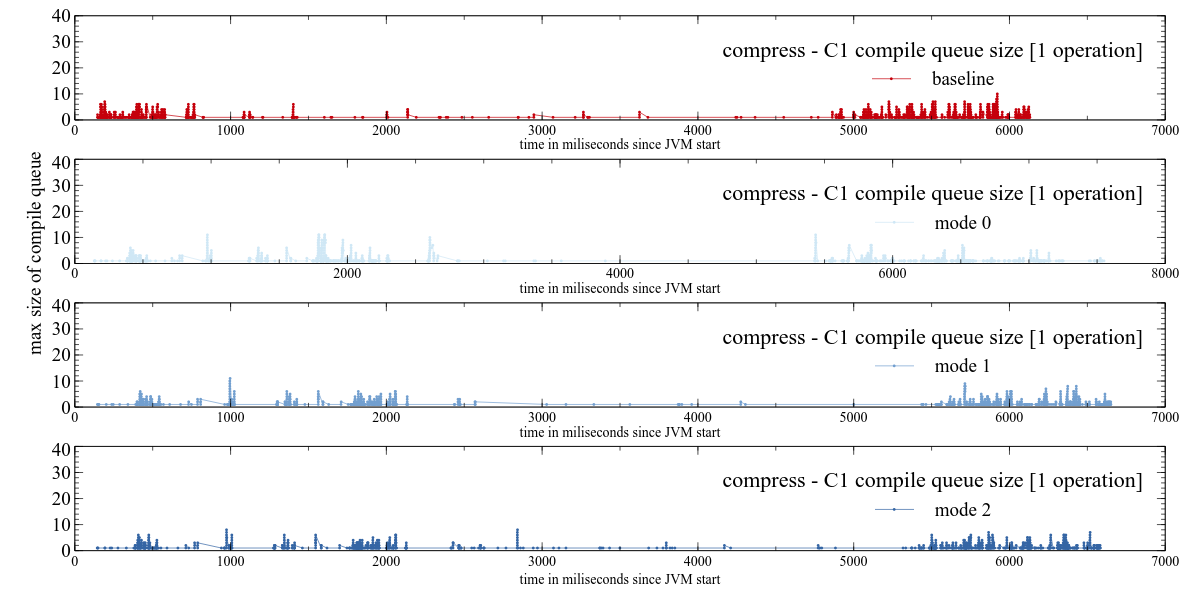
\includegraphics[width=0.90\textwidth]{figures/spec_queue_compress_separate_c1.png}
    \caption{C1 Compile queue size over time SPECjvm compress benchmark}
    \label{f:spec_queue_compress_separate_c1}
  \end{center}
\end{figure}
\begin{figure}[ht]
  \begin{center}
    \centering
    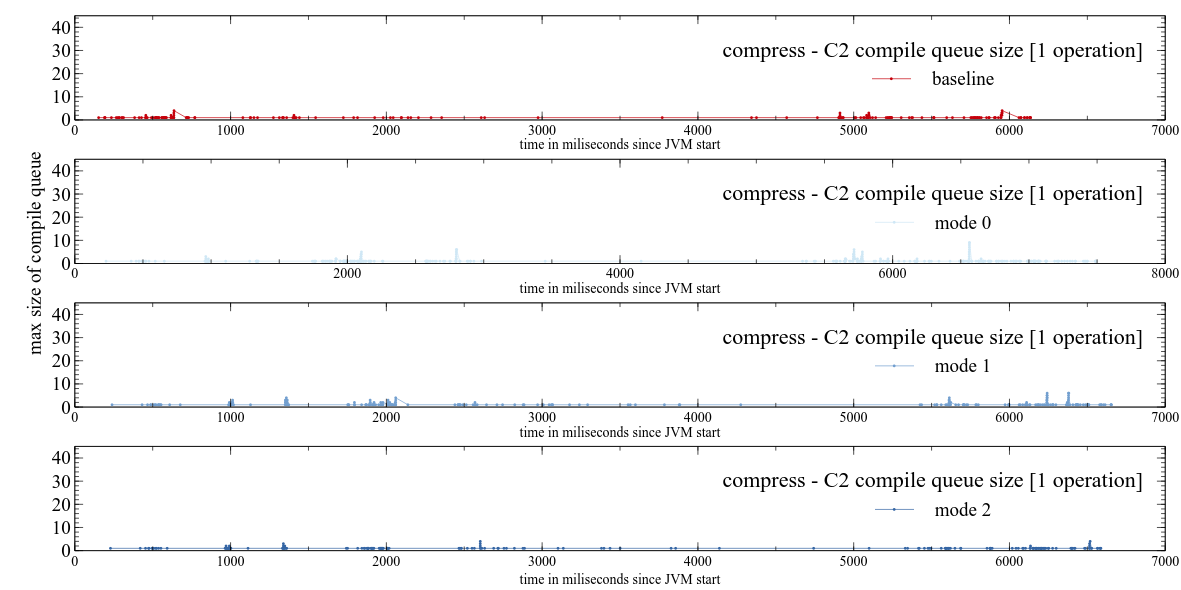
\includegraphics[width=0.90\textwidth]{figures/spec_queue_compress_separate_c2.png}
    \caption{C2 Compile queue size over time SPECjvm compress benchmark}
    \label{f:spec_queue_compress_separate_c2}
  \end{center}
\end{figure}
% --------------------------- SPECjvm scimark.sparse.large Queue ------------------
\begin{figure}[ht]
  \begin{center}
    \centering
    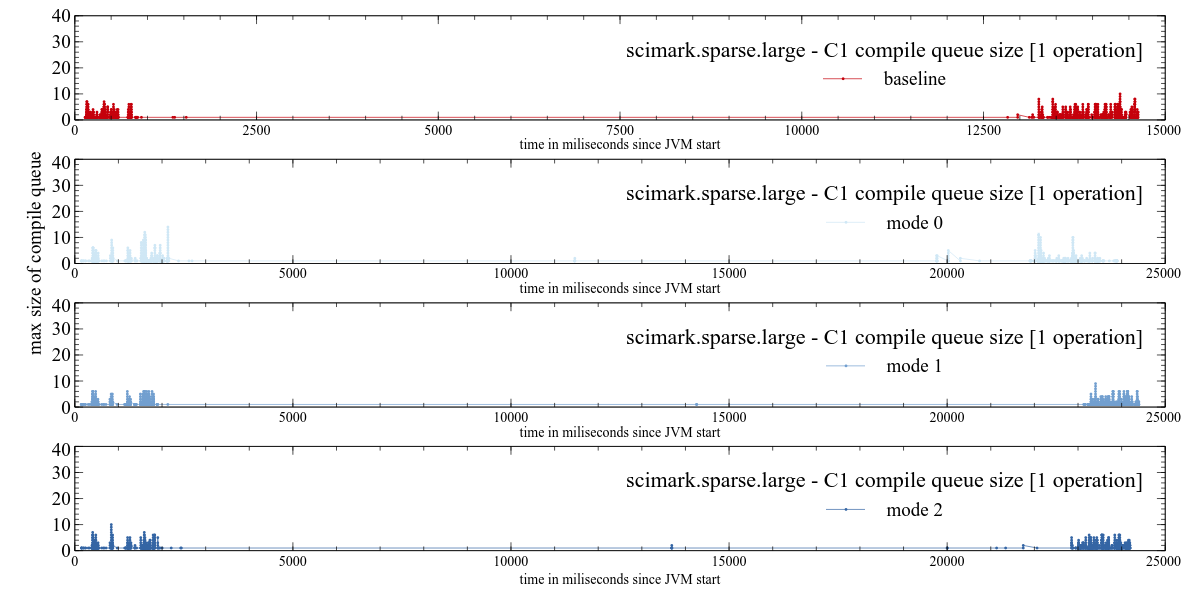
\includegraphics[width=0.9\textwidth]{figures/spec_queue_scirmarksparselarge_separate_c1.png}
    \caption{C1 Compile queue size over time SPECjvm scimark.sparse.large benchmark}
    \label{f:spec_queue_scirmarksparselarge_separate_c1}
  \end{center}
\end{figure}
\begin{figure}[ht]
  \begin{center}
    \centering
    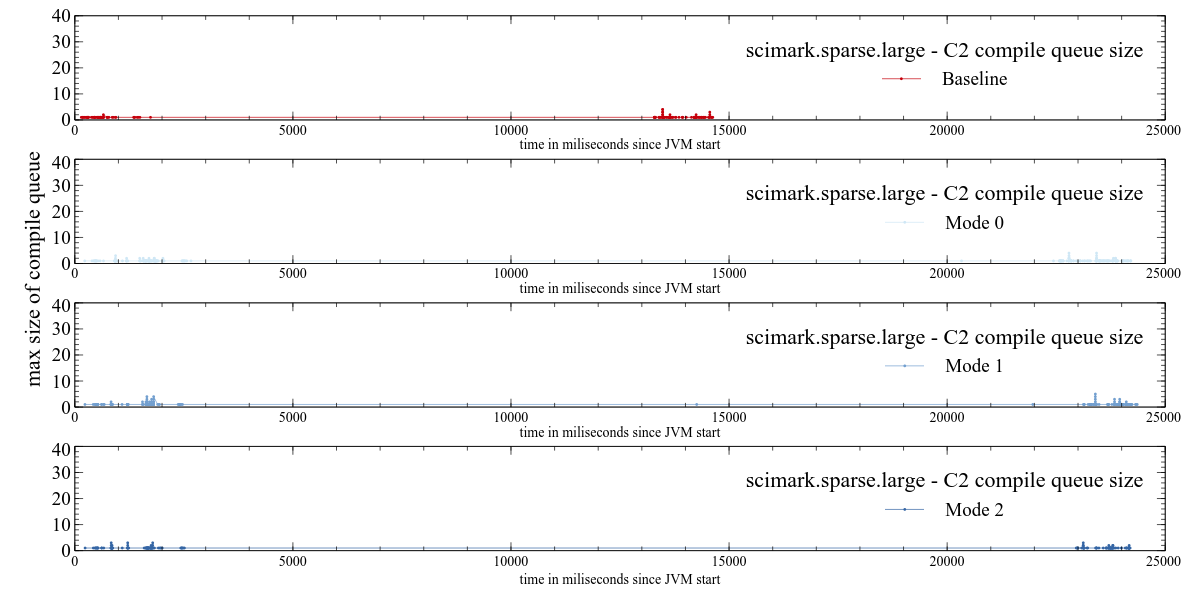
\includegraphics[width=0.9\textwidth]{figures/spec_queue_scirmarksparselarge_separate_c2.png}
    \caption{C2 Compile queue size over time SPECjvm scimark.sparse.large benchmark}
    \label{f:spec_queue_scirmarksparselarge_separate_c2}
  \end{center}
\end{figure}
